\begin{figure}[H]
  \begin{center}
    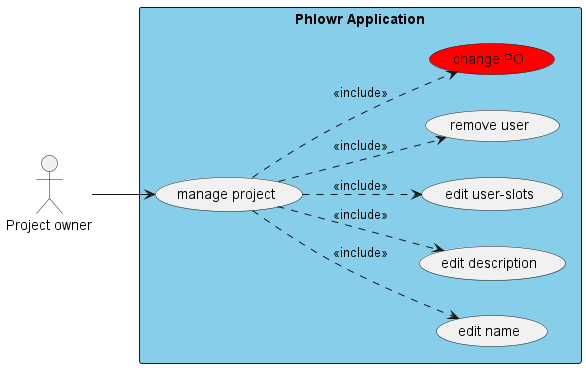
\includegraphics[width=0.3\linewidth]{../content/diagrams/usecase/manageProject/manageProjectUseCaseChangePOSelected.png}
    \caption{Use Case Diagaramm <change PO> }
  \end{center}
\end{figure}


\begin{table}[H]
    \centering
    \settowidth\tymin{executeIncomingCommand()}
    \setlength\extrarowheight{2pt}
    \begin{tabulary}{1.0\textwidth}{|m{4cm}|m{9cm}|}
      \hline
      \textbf{Use Case} &
      \textbf{CHANGE PO}\\
      \hline
      \textbf{Beschreibung} &
      Der Projekt-Owner des Projektes wird geändert\\ 
      \hline
      \textbf{Includes} &
      \begin{itemize}
       \item keine
        \end{itemize}\\  
        \hline
      \textbf{Akteure} &
      Projekt-Owner\\ 
      \hline
      \textbf{Auslöser} &
      Der Projekt-Owner soll geändert werden\\ 
      \hline
      \textbf{Vorbedingungen} &
      \begin{itemize}
        \item Vorbedingungen vom <MANAGE PROJECT>-Use-Case
        \item Der neue Projekt-Owner muss als User im Projekt registriert sein
      \end{itemize}\\  
      \hline
      \textbf{Abschlussbedingunen} &
      Der Projekt-Owner wurde geändert und die Änderungen sind gespeichert\\ 
      \hline
      \textbf{Ablauf} &
      \begin{enumerate}
        \item Applikation öffnen
        \item <Projekt Editieren> wählen
        \item <Change Project Owner> wählen
        \item Neuer PO aus liste der registrierten User auswählen
        \item Speichern
        \end{enumerate}\\ 
      \hline
      \textbf{Zu Beachten / Notizen} &
      \begin{itemize}
        \item Wird ein PO inaktiv, so kann das Projekt nicht mehr bearbeitet werden,
        der PO muss dann manuell im JSON-File geändert werden
        \end{itemize}\\ 
      \hline
    \end{tabulary}
    \caption{Use Case: manage project -> CHANGE PO}
  \end{table}
